\documentclass{article}
\usepackage[utf8]{inputenc}
\usepackage[english]{babel}
\usepackage{csquotes}
\usepackage[backend=biber,style=nature,sorting=ynt]{biblatex}
\usepackage{graphicx}
\usepackage{subcaption}
\addbibresource{mybib.bib}

\title{SUHII Project Internship Report}
\author{Michael Wang}
\date{September 2019}

\begin{document}

\maketitle

\section{Objective}

The objective of this internship project was to derive the surface urban heat island intensity of cities in the TraK project by implementing the method from Li, et al. 2018 \cite{li_new_2018} on Google Earth Engine.

\section{Data and Methods}
The intensity of the surface urban heat island usually refers to the difference in land surface temperature (LST) between non-urban and urban locations.
The novelty of Li et al. 2018 \cite{li_new_2018} lies in the fact that it uses the documented relationship between LST and impervious surface areas (ISA) to fit a line between LST and ISA as a percent (\%ISA). The slope of the resulting line would have the equation:
\[f(x) = mx + b\]
\[\Downarrow\]
\[f_{LST}(\%ISA) = m(\%ISA) + ISA_{0\%}\]

Where m is the slope of the line. 

Since the intensity of the urban heat island (SUHII) can be defined as the surface temperature difference between urban and non-urban areas:

\[SUHII = f_{LST}(100) - f_{LST}(0) \]
\[\Downarrow\]
\[SUHII = (100m +  ISA_{0\%}) - (0m +  ISA_{0\%})\]
\[\Downarrow\]
\[SUHII = 100m\]

Thus SUHII is simply the slope of the fitted line multiplied by a constant of 100.
The following data was used to derive this value for each city:
\begin{itemize}
    \item A vector file of the region of interest (ROI)
    \item The World Settlement Footprint (WSF) 2015 data from DLR
    \item Landsat-derived Land Surface Temperature data from Parastatidis \cite{parastatidis_online_2017}
    \item JRC Global Surface Water Mapping Layers v1.1 from the European Commission/Google \cite{pekel_high-resolution_2016}
\end{itemize}

 The ISA data was first processed using the kernel density estimation (KDE) technique, which was applied to account for the radiance effect of impervious surfaces, where the heat of an impervious pixel is not entire contained within, as it also radiates outward into other pixels. The temperature derived from the satellite LST data, would reflect effect, thus KDE was used to account for it. The specific radius of used for the KDE will affect the results (see section 4), but a radius of 3000 meters was used in line with the original paper. Afterwards, the entire image is normalized, such that 100\% ISA refers to the most impervious areas, and 0\% the least:
 
 \[normalized = \frac{pixelvalue - minvalue}{maxvalue - minvalue}\]

The LST data is averaged at the 1km level and stacked with the max extent binary water data which was aggregated at the 1km level for a percentage. The ISA layer is then averaged at the 1km level and stacked with the other two layers. The entire stack is then clipped to the ROI, and pixels where there is more than 25\% water is removed from further analysis due to the particular thermodynamics of water.

The pixels are then grouped using the ISA layer at 2\% intervals, creating 50 "buckets" of data. This particular application did this by dividing each percentage by 2 and applying a floor function, before returning to the original range by multiplying by 2 again. For each bucket, the associated LSTs are averaged. Then a CSV with two columns is exported, with one with \%ISA at 2\% intervals, the other being the average LST for that particular interval.

The slope of the first order linear regression of these two variables would give the SUHII per the original method. For each city, the a different SUHII was derived for the summer months (May-September), winter months (October-April), and annually.

\section{Results}
The resulting files are then analyzed and visualized with python. A selection of results are shown here: 

\begin{figure}[!htb]
    \begin{subfigure}{0.333\textwidth}
        \centering
        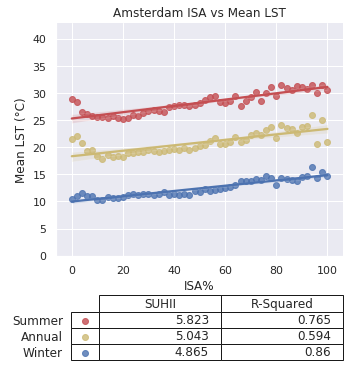
\includegraphics[width=1\linewidth]{Amsterdam3000.png}
        \caption{Amsterdam SUHII}
        \label{fig:subim1}
    \end{subfigure}\hfill
    \begin{subfigure}{0.333\textwidth}
        \centering
        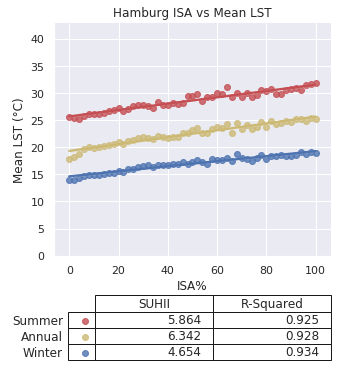
\includegraphics[width=1\linewidth]{Hamburg3000.png}
        \caption{Hamburg SUHII}
        \label{fig:subim2}
    \end{subfigure}\hfill
    \begin{subfigure}{0.333\textwidth}
        \centering
        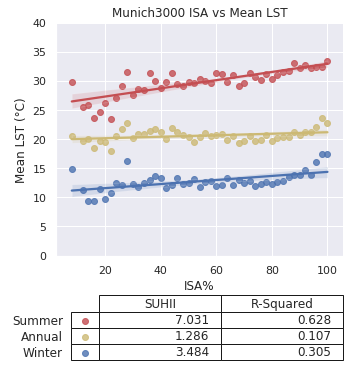
\includegraphics[width=1\linewidth]{Munich3000.png}
        \caption{Munich SUHII}
        \label{fig:subim3}
    \end{subfigure}
    \caption{A Selection of European City and the plotted \%ISA and LST}
    \label{fig:my_label}
\end{figure}

In general, the surface urban heat island effect is less intense in winter than in summer, with the annual being somewhere in the middle. The coefficient of determination ($R^2$) was also higher in summer than in winter, meaning the variances are better explained by the fitted linear regression in summer than in winter.

The SUHII value of each season for each city is appended to the original shape file as a new column through the use of geopandas.

\section{Discussion}
The $R^2$ of the fitted line varies greatly between cities, probably due to the heterogeneous and idiosyncratic nature of the urban landscape.

\subsection{The $R^2$ Sensitivity Test}



\section{Description of Delivered Data}
The shape files are g

\medskip

\printbibliography

\end{document}
